\chapter{Data Stratification}
\label{chapter:data_stratification}


In order to better understand the properties of the data in the \ac{iemo} dataset, we performed stratification based on several attributes of the dataset. The aim of this stratification was to group similar data together and investigate their common properties, and, discover limitations that these properties pose to the machine learning model in the \ac{ser} area.

\section{Recordings Durations}

The duration of an audio recording can significantly impact the analysis and modeling of the data. Shorter recordings may not capture enough information to adequately represent the signal of interest, while longer recordings may contain irrelevant or redundant information.

We stratified the dataset based on the duration of the recordings. The dataset contains recordings ranging from approximately 0.25 to 34 seconds in duration, and we divided the recordings into three evenly balanced groups, in terms of number of recordings: short, less than or equal to  2.29 seconds, medium, greater than 2.29 and less than or equal to 4.38 seconds, and long, greater than 4.38 seconds.

Table \ref{5:durations} presents the impact of the duration of the recordings on the performance of the chosen traditional AdaBoost model. The longest recordings have the highest performance, with an accuracy of 63.4\%, despite having more recordings than the medium duration data. 

\begin{table}[H]
	\centering
	\caption{Traditional Model 5-Fold Cross-Validation Results Based on the Recordings Duration.}
	\label{5:durations}
	\begin{tabular}{lrlrrrr}
		\toprule
		Recordings Duration &   Total Data & Accuracy    &   Macro F1 &   Precision &   Recall &   MCC. \\
		\midrule
		Short ($]0, 2.29]$ s)	 	&      1844 & 57.38+-1.15 &   55.48 &  59.51 &  53.88 &  0.40  \\
		Medium ($]2.29, 4.38]$ s) 	&      1843 & 56.38+-1.26 &   56.81 &  57.34 &  56.73 &  0.41 \\
		Long ($]4.38, 34]$ s) 		&      1844 & 62.91+-1.69 &   63.31 &  63.91 &  63.11 &  0.50  \\
		
		
		\bottomrule
	\end{tabular}
\end{table}

The obtained classification results suggest that longer recordings are easier for the model to classify accurately, as they provide more information. This allows us to conclude that recordings' duration has a substantial performance impact on the \ac{ser} task and is a significant factor to consider when building classification models.

\section{Speaker Gender}

Another attribute we used for stratification was the gender of the speaker. The dataset contains a similar amount of recordings from both male and female speakers, having 2649 recordings with female speakers and 2882 with male speakers.

To evaluate the performance of the model on different genders, we trained and tested the model on recordings from female speakers, male speakers, and mixed-gender recordings. Table \ref{5:gender} shows the 5-fold cross-validation results of the model on each category.

\begin{table}[H]
	\centering
	\caption{Traditional Model 5-Fold Cross-Validation Results Based on Speaker Gender Recordings.}
	\label{5:gender}
	\begin{tabular}{llrrrrr}
		\toprule
		Training Gender & Testing Gender & Accuracy    &   Macro F1 &   Precision &   Recall &   MCC. \\
		\midrule
		Female	& Female & 59.87+-1.03 & 60.45 & 60.55 & 60.77 & 0.46 \\
		Male 	& Male	 & 59.92+-1.33 & 60.43 & 61.66 & 59.72 & 0.45 \\
		Female  & Male	 & 51.49+-1.38 & 51.55 & 53.67 & 51.52 & 0.33 \\
		Male    & Female & 51.45+-1.76 & 52.01 & 55.35 & 51.23 & 0.35 \\
		\bottomrule
	\end{tabular}
\end{table}

From the table, it can be observed that the model performed similarly on both genders, when the testing data for the model is of the training data, with accuracies close to 60\%. However, when testing with different speaker gender, the model's accuracy dropped significantly to 51.49\% and 51.45\% for female and male training data, respectively. The other metrics showed equivalent behavior, indicating difficulty in correctly identifying the emotion in mixed-gender contexts.

These results suggest that the model's performance is affected by the gender of the speakers in the training data and therefore, it is important that the model is provided a gender-balanced set of training data to reduce gender bias.

\section{Discrete Emotions}

The \ac{iemo} dataset contains four emotional categories: anger, happiness, sadness, and neutral. We stratified the data based on these labels and obtained 15 groups of data. In this section, we discuss the differences in classification performance between these emotional categories, as well as differences in valence and emotional plane.


Table \ref{tab:emo_cat} shows the traditional model 5-fold cross-validation results based on the discrete emotions. In the four-label case, which includes all four emotional categories, the model achieved an accuracy of 60.04\% with a macro F1 score of 60.76. The best performance was achieved when classifying between anger, happiness, and sadness, with an accuracy of 70.36\% and a macro F1 score of 70.73. The worst performance was achieved when classifying between angry, neutral, and happy, with an accuracy of 64.4\% and a macro F1 score of 63.8.


\begin{table}[H]
\small
\centering
\caption{Traditional Model 5-Fold Cross-Validation Results Based on the Discrete Emotions.}
\label{tab:emo_cat}
    \centering
    \begin{tabular}{lrrrrrr}
    	\toprule
    	Labels                      &   Total Data & Accuracy    & Macro F1    & Precision   & Recall      & MCC.       \\
    	\midrule
 	    \multicolumn{7}{c}{Four Labels} \\
    	Angry, Happy, Sad, Neutral             &         5531 &  60.04$\pm$0.95 & 60.76 & 61.29 & 60.59 & 0.459 \\
    	\midrule
    	\multicolumn{7}{c}{Three Labels} \\
    	
		Angry, Happy, Sad                   &         3823 & 70.36$\pm$1.09 &      70.73 &       71.36 &    70.35 &   0.54 \\
		Angry, Neutral, Happy               &         4447 & 64.4$\pm$0.95  &      63.8  &       64.48 &    63.84 &   0.46 \\
		Angry, Neutral, Sad                 &         3895 & 74.02$\pm$1.14 &      74.16 &       75.61 &    73.2  &   0.6  \\
		Sad, Neutral, Happy                 &         4428 & 65.4$\pm$1.12  &      65.59 &       65.75 &    65.54 &   0.47 \\
		
		Sad, Neutral, Happy+Angry (Arousal or Dominance) &         5531 & 68.54$\pm$1.03 &      66    &       66.31 &    65.89 &   0.49 \\
		Angry+Sad, Neutral, Happy (Valence) &         5531 & 60.15$\pm$0.86 &      58.94 &       59.53 &    58.99 &   0.39 \\
    	\midrule
    	\multicolumn{7}{c}{Two Labels} \\
    	    	
    	Angry, Sad                          &         2187 & 91.4$\pm$1.46  &      91.4  &       91.46 &    91.39 &   0.83 \\
    	Angry, Neutral                      &         2811 & 84.13$\pm$0.88 &      82.98 &       84.03 &    82.34 &   0.66 \\
    	Angry, Happy                    	&         2739 & 74.66$\pm$2.01 &      73.1  &       73.84 &    72.72 &   0.47 \\
    	Sad, Neutral                        &         2792 & 79.51$\pm$1.57 &      77.98 &       78.77 &    77.49 &   0.56 \\
    	Sad, Happy                          &         2720 & 83.6$\pm$1.41  &      82.87 &       82.93 &    82.82 &   0.66 \\
    	Neutral, Happy                      &         3344 & 72.58$\pm$2.38 &      72.43 &       72.81 &    72.45 &   0.45 \\
    	Sad+Neutral, Happy+Angry (Arousal or Dominance)  &         5531 & 77.2$\pm$1.29  &      77.18 &       77.25 &    77.18 &   0.54 \\
    	Angry+Sad, Neutral+Happy (Valence)  &         5531 & 72.86$\pm$0.94 &      69.84 &       72.47 &    69.27 &   0.42 \\
    	\bottomrule
    \end{tabular}
\end{table}

In the two-label case, where the emotional categories were paired, the best performance was achieved when classifying between angry and sad, with an accuracy of 91.4\% and a macro F1 score of 91.4. The worst performance was achieved when classifying between angry+sad and neutral+happy based on valence, with an accuracy of 72.86\% and a macro F1 score of 69.84.

In terms of valence and emotional plane, the model achieved its highest accuracy (68.54\%) when classifying between sad, neutral, and happy+angry based on arousal, and its lowest accuracy (60.15\%) when classifying between angry+sad, neutral, and happy based on valence. These results suggest that the model is better at distinguishing emotional categories based on arousal than valence.

It is important to note that the total data impacts the classification, as a lower number of files may make the classification easier. However, even with a large dataset such as \ac{iemo}, the performance of the model varied widely depending on the emotional categories and valence or arousal being classified. These results have implications for the development of affective computing systems, which must take into account the nuances of emotional categorization and valence/arousal classification in order to accurately interpret and respond to human affect.


\section{Dimensional Emotions}

In addition to the categorical classification, we also explored the dimensional annotations of the dataset in terms of valence (ranging from unpleasant to pleasant), arousal (ranging from calm to excited), and dominance (ranging from submissive to dominant). These dimensions were rated on a continuous scale of 1 to 5 by human judges.

Initially, we aimed to investigate the level of difficulty associated with classifying each emotional dimension, so we utilized traditional approach features to assess the performance of a Random Forest Regressor model from sklearn for each dimension. Each dimension underwent 5-fold cross-validation. We used MAE, RMSE, and $R^2$ as evaluation metrics for the model.

Table \ref{tab:dim_reg} shows the results of our experiments on the regression task. The arousal and dominance dimensions are easier to classify than valence. One possible reason for this is that valence is a more complex and abstract concept that may be more difficult to recognize and classify in speech. Additionally, the annotations for valence may be more subjective and varied among annotators than the others, leading to less reliable labels and lower classification performance.


\begin{table}[H]
	\centering
	\caption{Random Forest Regressor 5-Fold Cross Validation using Dimensional Emotions as Labels.}
	\label{tab:dim_reg}
	\begin{tabular}{lrrr}
		\toprule
		Regression Labels   &   MAE &  RMSE & $R^2$ \\
		\midrule
		Valence             & 0.700 & 0.859 & 0.182 \\
		Arousal             & 0.414 & 0.522 & 0.520 \\
		Dominance           & 0.534 & 0.657 & 0.362 \\
		\bottomrule
	\end{tabular}
\end{table}

We conducted a comparison between the discrete and dimensional annotations by calculating the means of each dimensional label based on the discrete one. These means, known as dimensional centroids, are presented in Table \ref{tab:dis_dim} and a in 2D plane \ref{fig:2dplane}. To determine if the centroids are accurate or too distant from the expected values, we compared them with the state-of-the-art Russell and Mehrabian's \ac{vad} model.

\begin{table}[H]
	\centering
	\caption{Discrete Emotions' Means of the Dimensional Annotations and Comparison to the \ac{vad} model.}
	\label{tab:dis_dim}
	\begin{tabular}{lrrr}
		\toprule
		Emotion & Mean Arousal &   Mean Valence & Mean Dominance \\
		\midrule
		VAD Anger     & 4.34 & 2.14 & 3.68 \\
		VAD Happiness & 3.96 & 4.52 & 3.70 \\
		VAD Neutral   & 3.00 & 3.00 & 3.00 \\
		VAD Sadness   & 3.54 & 1.74 & 2.34 \\
		\addlinespace
		Anger   	&   3.64 \textcolor{red}{$(-0.70)$} &  1.91 \textcolor{red}{$(-0.23)$} &  3.95 \textcolor{green}{$(+0.27)$} \\
		Happiness   &   3.41 \textcolor{red}{$(-0.55)$} &  3.95 \textcolor{red}{$(-0.57)$} &  3.23 \textcolor{red}{$(-0.47)$} \\
		Neutral 	&   2.73 \textcolor{red}{$(-0.27)$} &  2.97 \textcolor{red}{$(-0.03)$} &  2.83 \textcolor{red}{$(-0.17)$} \\
		Sadness     &   2.56 \textcolor{red}{$(-0.98)$} &  2.25 \textcolor{green}{$(+0.51)$} &  2.83 \textcolor{green}{$(+0.49)$} \\
		\bottomrule
	\end{tabular}
\end{table}

teste

\begin{figure}[H]
  \centering
  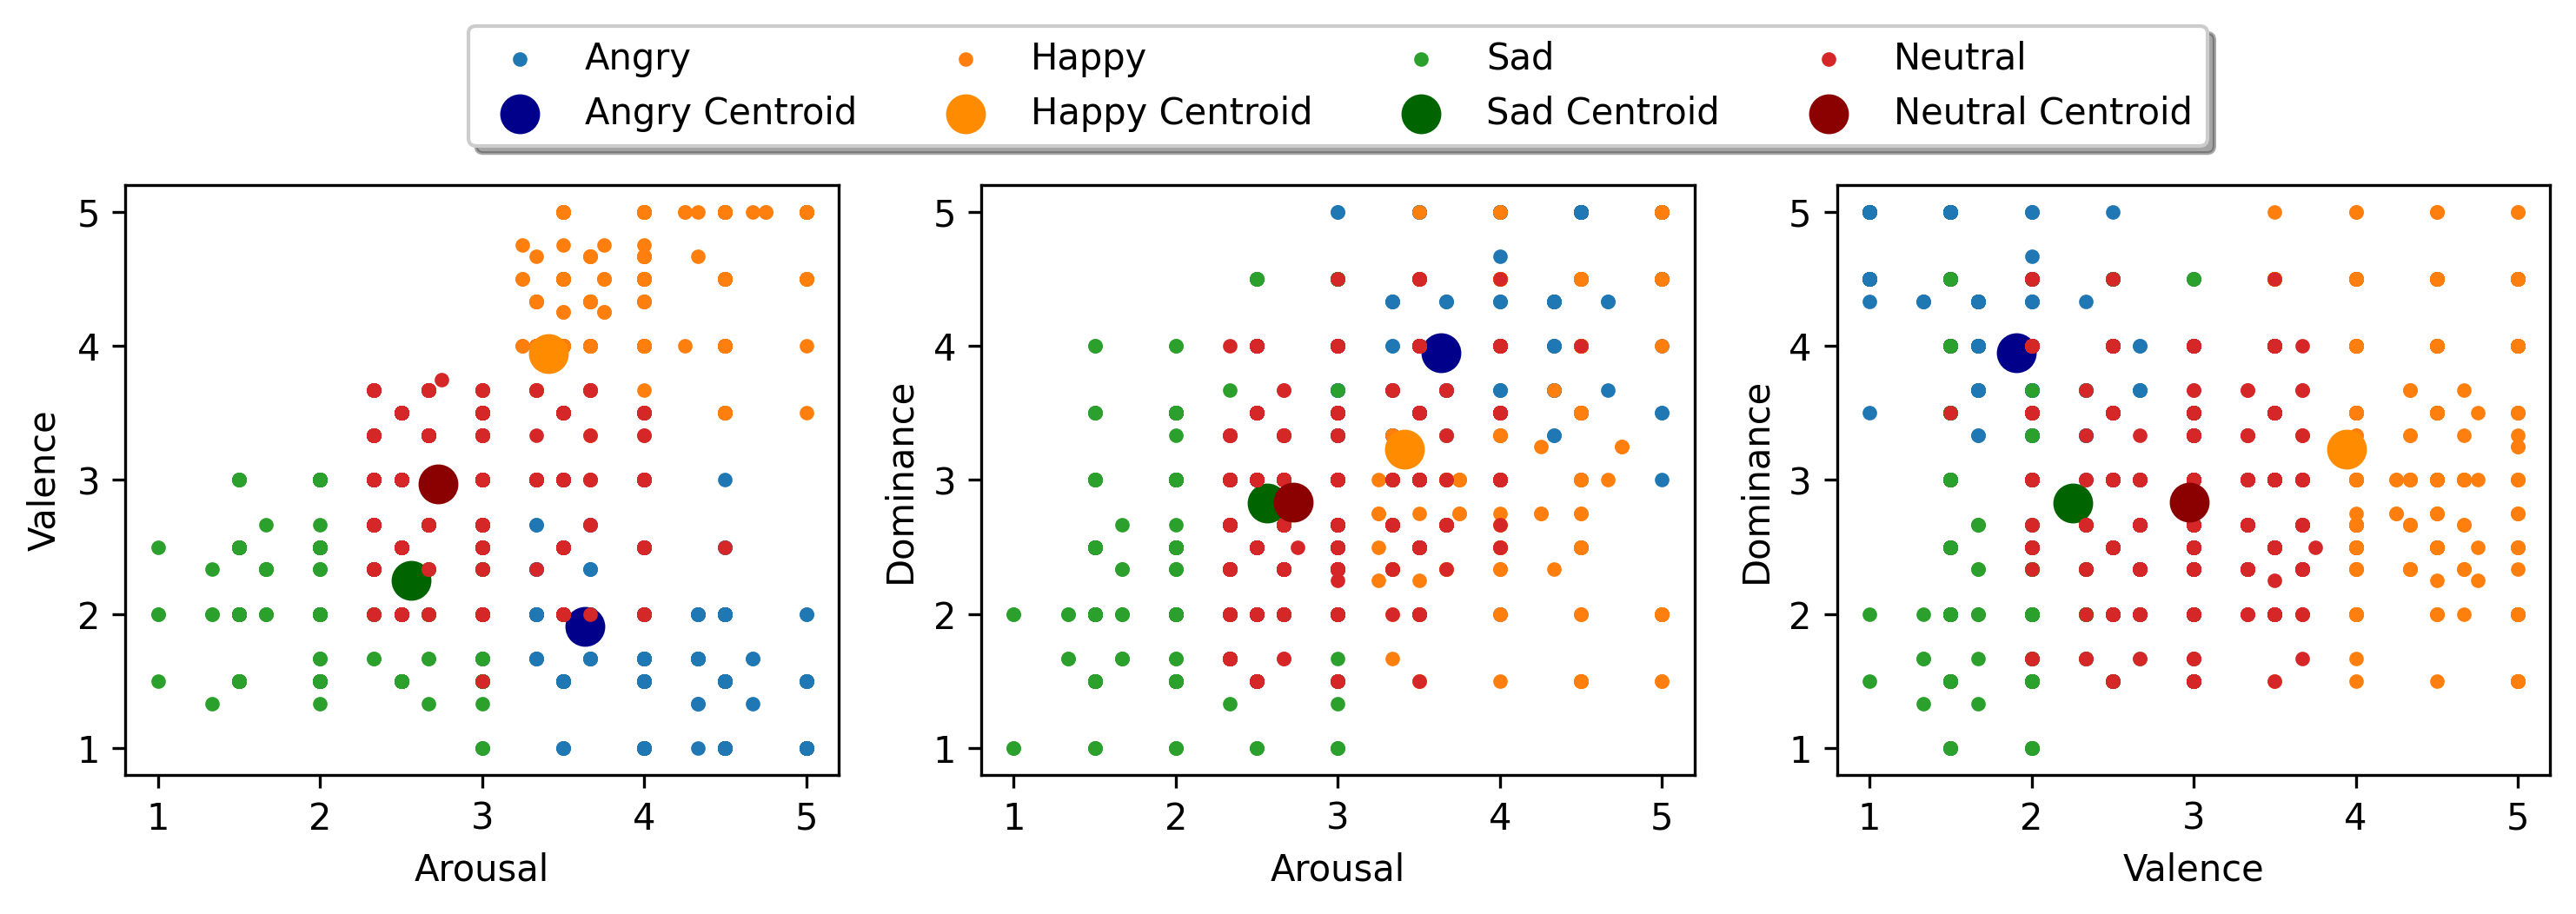
\includegraphics[width=.9\linewidth]{figs/5_data_stratification/primitives_visualization_2d.png}
  \caption{2D representation of \ac{iemo} dimensional emotions and the \ac{vad} model centroids.}
  \label{fig:2dplane}
\end{figure}

The results indicate that the centroids of each discrete emotion have some differences to the \ac{vad} model. For the arousal dimension, it was noted that all emotions have lower values, with sadness showing a greater deviation. In terms of valence, the annotations are more comparable to the \ac{vad} model, but sadness contradicts the lower trend of the other two emotions. The annotations on the dominance dimension also vary the deviations trends.

Based on this, we decided to remove any data that contains dimensional annotations far from the \ac{vad} model centroids for each discrete emotion. Table \ref{tab:conf} demonstrates this conflicts removal process between each emotion's categories and the respective dimensional annotations.

\begin{table}[H]
\caption{Maintained Dimensional Annotations Range For Each Emotion Category.}
\label{tab:conf}
\centering
    \begin{tabular}{lrrr}
        \toprule
        {} & \multicolumn{3}{c}{Dimensions} \\ \cmidrule{2-4}
        Emotion Categories &    Arousal &      Valence &       Dominance \\
        \midrule
        Angry   &   $]2, 5]$  	& $[1, 4.5]$ 	&  None 		\\
        Happy 	&   $[2.5, 5]$  & $[3, 5[$ 		&  None 		\\
        Sad    	&   $]2, 5]$ 	& $[1, 4]$ 		&  $[1, 4]$ 	\\
        Neutral &   $]2, 4[$	& $[2, 4]$ 		&  $]2, 4[$		\\
        \bottomrule
    \end{tabular}
\end{table}


With this process, 1136 audio files were removed, having now 4395 audio files and the new centroids were calculated again, as table \ref{tab:new_c} shows.


\begin{table}[H]
	\centering
	\caption{Discrete Emotions' Means of the Dimensional Annotations and Comparison to the \ac{vad} model after Conflicts Removal Process.}
	\label{tab:new_c}
	\begin{tabular}{lrrr}
		\toprule
		Emotion & Mean Arousal &   Mean Valence & Mean Dominance \\
		\midrule
		Anger   	&   3.66 \textcolor{red}{$(-0.68)$} &  1.91 \textcolor{red}{$(-0.23)$} &  3.95 \textcolor{green}{$(+0.27)$} \\
		Happiness   &   3.47 \textcolor{red}{$(-0.49)$} &  4.02 \textcolor{red}{$(-0.50)$} &  3.26 \textcolor{red}{$(-0.44)$} \\
		Neutral 	&   2.86 \textcolor{red}{$(-0.14)$} &  2.97 \textcolor{red}{$(-0.03)$} &  2.93 \textcolor{red}{$(-0.07)$} \\
		Sadness     &   2.87 \textcolor{red}{$(-0.67)$} &  2.25 \textcolor{green}{$(+0.51)$} &  2.91 \textcolor{green}{$(+0.57)$} \\
		\bottomrule
	\end{tabular}
\end{table}


\begin{figure}[H]
  \centering
  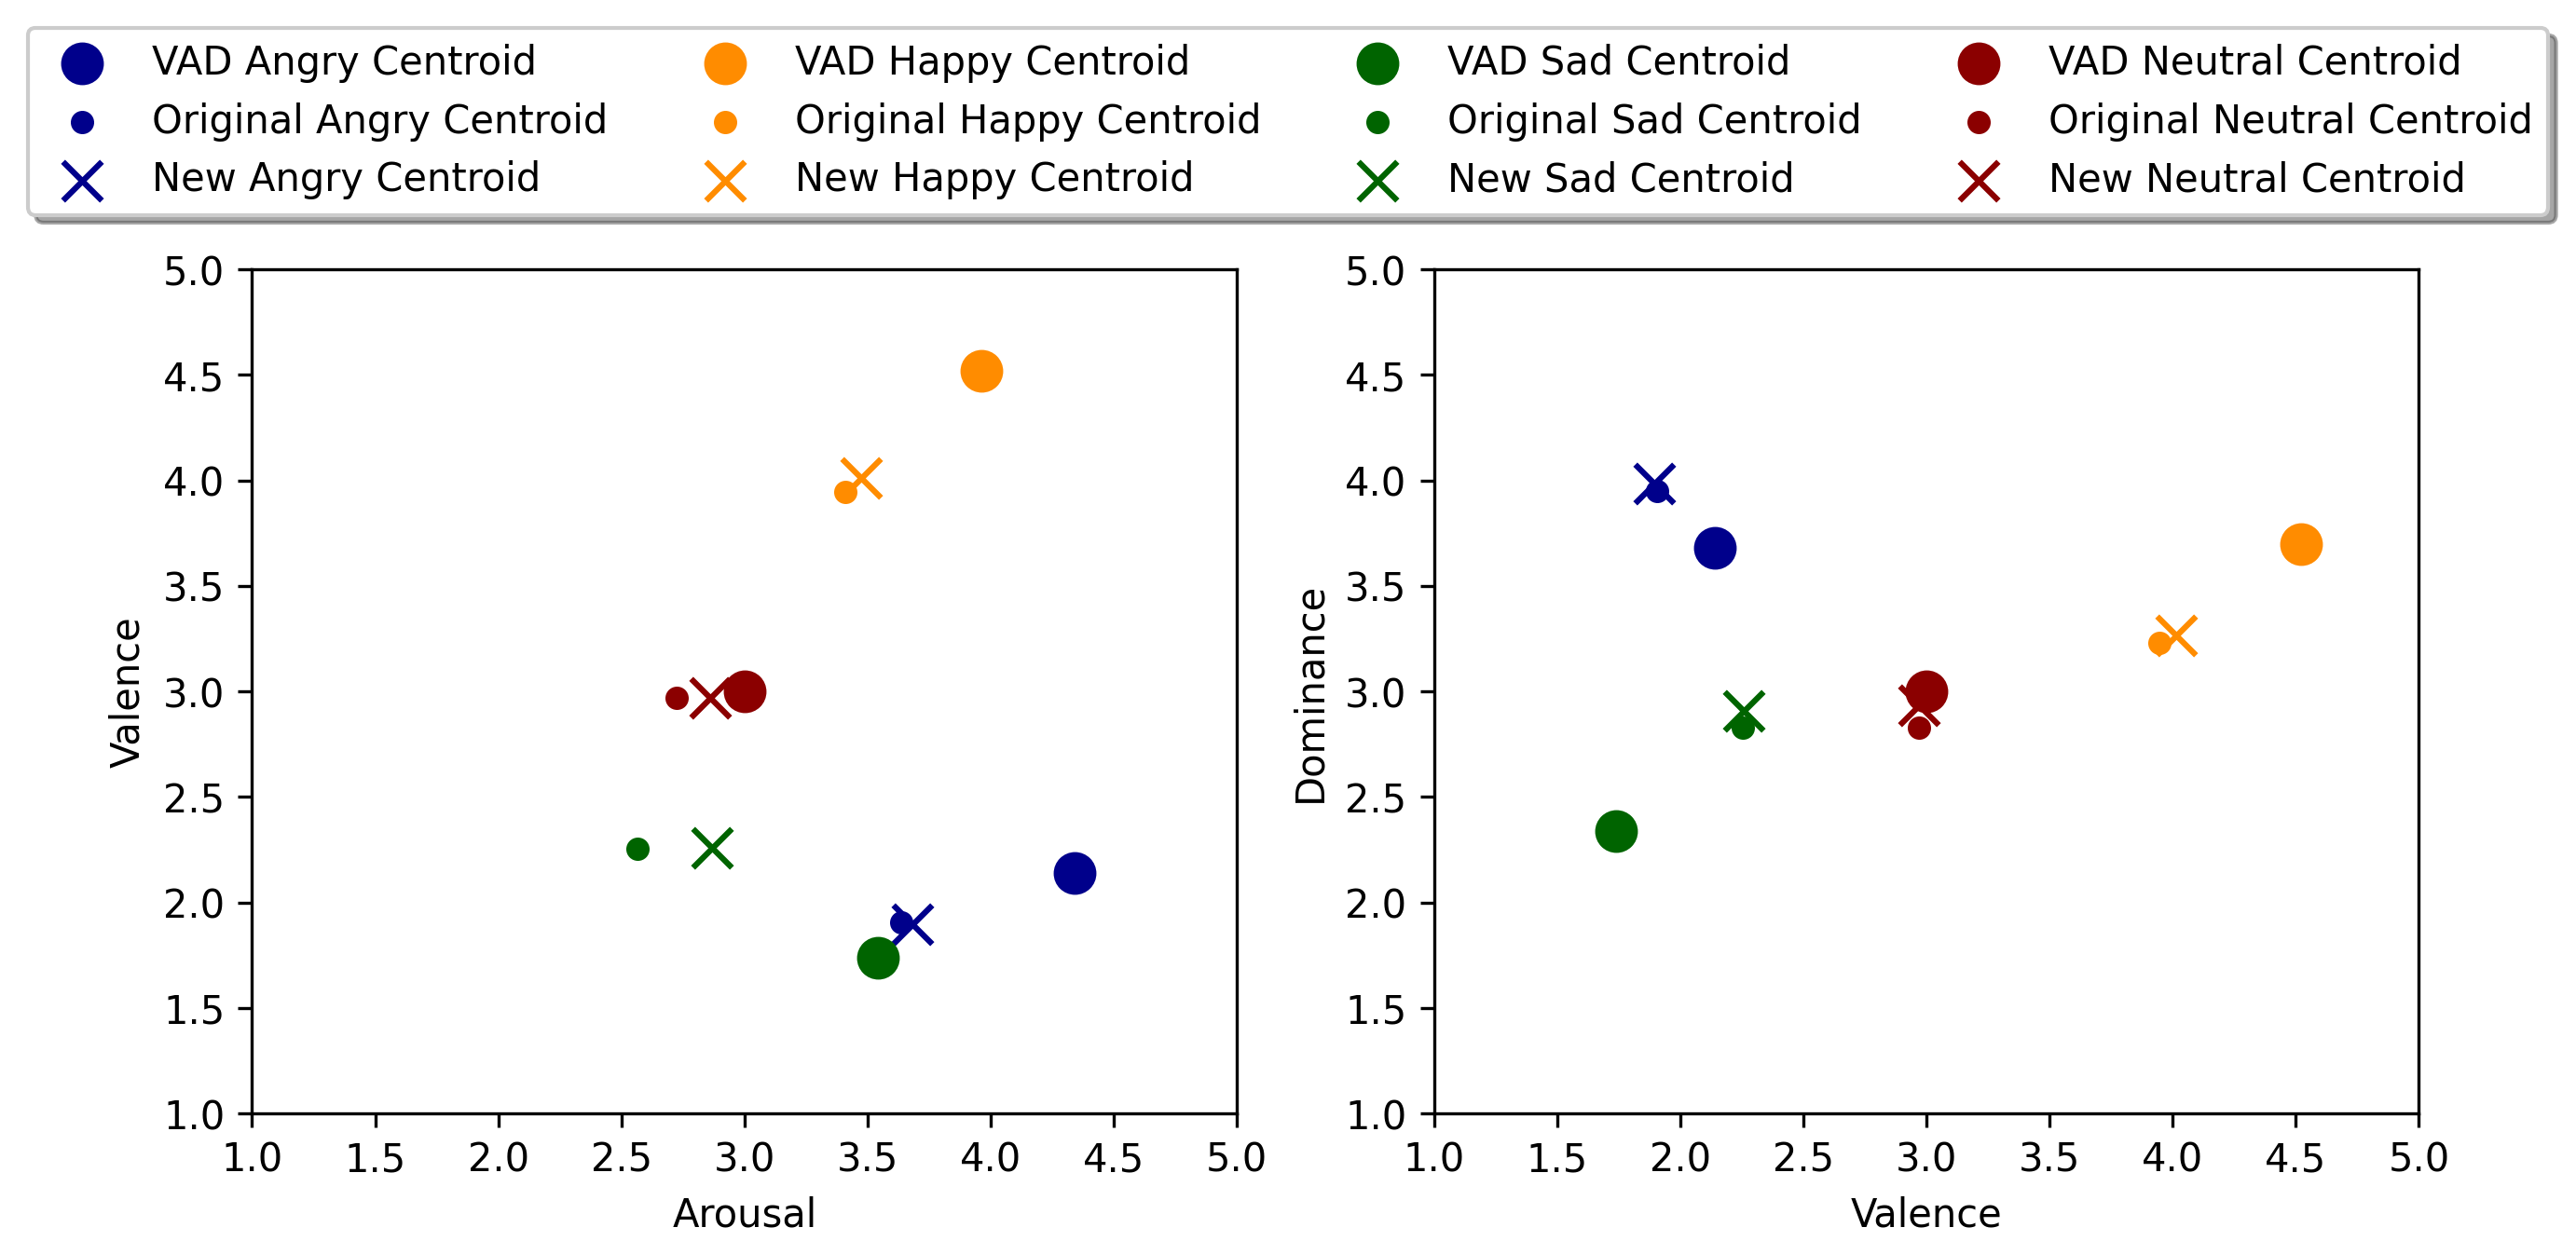
\includegraphics[width=.9\linewidth]{figs/5_data_stratification/strict_conflicts_centroids_2d.png}
  \caption{Data with and without conflicts between emotion's categories and primitives emotion centroids' 2D visualization}
  \label{fig:signalWP}
\end{figure}



\begin{table}[H]
	\small
	\centering
	\caption{Traditional Model 5-Fold Cross-Validation Results With Conflicts Removal Process.}
	\label{tab:emo_cat2}
	\centering
	\begin{tabular}{lrrrrr}
		\toprule
		Data   						 	& Accuracy    & Macro F1    & Precision   & Recall      & MCC.       \\
		\midrule
		All Data - 5531 Files		 	& 60.04$\pm$0.95 & 60.76 & 61.29 & 60.59 & 0.459 \\
		Conflict-Free Data - 4395 Files & 61.64$\pm$1.09 & 62.08 & 62.36 & 62.35 & 0.490 \\
		\bottomrule
	\end{tabular}
\end{table}


\subsection{Conclusion}

The data stratification process enabled us to uncover the shortcomings of the \ac{iemo} dataset and the model we developed. Having obtained valuable insights from our observations and conclusions on the subsections about duration, gender, and dimensional annotations, we aim to utilize the training data in our model to enhance its reliability and performance. In light of this, we have made the decision to train both traditional and deep learning models on data that aligns with our objectives.

To achieve this, to the conflict-free data obtained from the dimensional conflict removal process, we applied an additional file duration condition. Specifically, we only retained audio files with a duration exceeding 1 second, as it was necessary to ensure the presence of sufficient emotional data for the model to learn effectively. As a result of this process, we obtained a total of 4200 audio files, with a nearly balanced gender distribution, comprising 52.9\% male and 47.1\% female speakers.

Table \ref{tab:emo_cat3} presents the 5-fold cross-validation results of the traditional model trained on the \ac{iemo} dataset with different sets of selected data. The first row shows the results obtained with all 5531 files of the dataset. The second row shows the results after applying the dimensional conflict removal process, resulting in 4395 files. The third row shows the results of the conflict-free data with the previous mentioned additional duration condition, resulting in 4200 audio files. The results demonstrate that the performance of the traditional model improves as the data selection process becomes more rigorous. The dimensional conflict removal process resulted in an increase in accuracy from 60.04\% to 61.64\%, while the additional duration condition further improved the accuracy to 62.17\%, the other metrics also have the same behavior, indicating that the model's classification ability improved with the use of cleaner and more reliable data.

\begin{table}[H]
	\small
	\centering
	\caption{Traditional Model 5-Fold Cross-Validation Results With Conflicts Removal Process.}
	\label{tab:emo_cat3}
	\centering
	\begin{tabular}{lrrrrr}
		\toprule
		Data   						 	& Accuracy    & Macro F1    & Precision   & Recall      & MCC.       \\
		\midrule
		All		      & 60.04$\pm$0.95 & 60.76 & 61.29 & 60.59 & 0.459 \\
		Conflict-Free & 61.64$\pm$1.09 & 62.08 & 62.36 & 62.35 & 0.490 \\
		Conflict-Free With Duration Condition & 62.17$\pm$0.60 & 62.59 & 62.84 & 62.81 & 0.500 \\
		\bottomrule
	\end{tabular}
\end{table}

Removing conflicts from the dataset results in better performance metrics for our models, however, this approach comes reduces the amount of data which may be the reason for this improvements. To verify if the model does in fact improve, we decided to train and save both traditional and deep learning models with the data that met our set of conditions. These saved models are called stratified models. We then repeated the process made on the previous section and evaluated them on three different datasets, namely eNTERFACE'05, CREMA-D, and EMO-DB.

As shown in Table \ref{strat_final_models}, the stratified models outperformed the previous models trained on all of the \ac{iemo} data on most metrics, which demonstrate that our stratification study resulted in improved cross-dataset performance of the models.

\begin{table}[H]
	\centering
	\caption{Final models trained on \ac{iemo} and evaluated on different datasets.}
	\label{strat_final_models}
	\resizebox{\textwidth}{!}{%
		\begin{tabular}{llrrrrrr}
			\toprule
			Dataset & Model & Accuracy & Macro F1 & Precision & Recall & \ac{mcc} & Time \\
			\midrule
			
			eNTERFACE'05 & Traditional & 29.37 & 18.61 & 17.85 & 22.02 & 0.064 & 0.14 \\
			& Stratified Traditional & 29.68 & 18.82 & 40.7 & 22.26 & 0.025 & 0.14 \\
			& Deep Learning & 36.67 & 22.91 & 44.36 & 27.50 & 0.087 & 0.25 \\
			& Stratified Deep Learning & 37.14 & 22.39 & 43.51 & 27.86 & 0.073 & 0.24 \\

			\addlinespace			
			EMO-DB & Traditional & 38.94 & 17.36 & 25.75 & 26.72 & 0.087 & 0.11 \\
			& Stratified Traditional & 40.41 & 20.24 & 31.93 & 28.61 & 0.126 & 0.12 \\
			& Deep Learning & 38.35 & 15.79 & 37.78 & 25.99 & 0.066 & 0.18 \\
			& Stratified Deep Learning & 38.05 & 15.22 & 34.71 & 25.63 & 0.052 & 0.20 \\
			
			\addlinespace
			CREMA-D & Traditional & 44.41 & 35.45 & 63.18 & 46.12 & 0.335 &  0.11 \\
			& Stratified Traditional & 45.12 & 37.50 & 36.46 & 46.54 & 0.323 & 0.10 \\
			& Deep Learning & 54.14 & 47.71 & 51.68 & 52.98 & 0.407 & 0.20 \\
			& Stratified Deep Learning & 55.29 & 50.06 & 54.11 & 54.05 & 0.417 & 0.19 \\

			\bottomrule
		\end{tabular}%
	}
\end{table}

